\documentclass{article} % For LaTeX2e
\usepackage{cos424,times}
\usepackage{url}
\usepackage{graphicx}
\usepackage{hyperref}
\usepackage{array}
\usepackage{tabu}
\usepackage{cos424,times}
\usepackage{cite}
\usepackage{amsmath}
%\usepackage{natbib}
\usepackage{multirow}
\usepackage{bm,bbm}
 \usepackage{amssymb}
\usepackage{amsmath}
\usepackage{wrapfig}
\usepackage{float}
\usepackage{caption}
\usepackage{subcaption}

\title{Classification of review sentiments}


\author{
Rediet Tilahun Desta\\
Department of Electrical Engineering\\
\texttt{rtilahun@princeton.edu} \\
}

\newcommand{\fix}{\marginpar{FIX}}
\newcommand{\new}{\marginpar{NEW}}

\begin{document}

\maketitle

\begin{abstract}
In this age where we mostly buy products be they clothes or music, we would like to get the opinions of others before making the decision. However going through all reviews can be time consuming. Companies that faciliate this trading process would like to present their customers with a quick and easy way to gauge the overall response to the product; the first step of which will be analyzing the sentiments of each reviews. In this assignment, I attempt to find a good sentiment classifier which would classify reviews as either positive or negative, using a data set of 3000 reviews. I employed Natural Language Processing(NLP) techniques to represent the data as a bag-of-words which were then used to train six types of classifiers.  Almost all classifiers performed really well: having similar and high values of precision and recall. The real difference was in the computational time at which multinomial and bernoulli naive bayes classifiers significantly outperformed the rest more complex classifiers while still maintaing a good precision and recall value. 
\end{abstract}

\section{Introduction}
Sentiment analysis used to be a very human task in the past. However in recent years, with the growth of online companies, the need for automated forms of sentiment analysis were found to be of most importance. Online companies like Amazon, Facebook, Twitter and Yelp are increasingly becoming dependent on machine learning algorithms to classify the sentiment of the billions of textual inputs they receive daily. In this assignment, I am interested in learning which type of classifiers perform well in classifying the sentiments of online reviews. Moreover, I want to gain the understanding of why certain classifiers perform well while others less so. 

I evaluate 6 types of classifiers in this report. In the feature extraction process, I chose unigrams and then in the feature selection component selected those unigrams that appear more than 5 times in the 2400 data set. Other feature selection techniques were also used and then compared as to their impact on classifier performance such as computational speed, precision and recall. 


\section{Related Work}
The first indepth analysis of the field of sentiment analyis and classification was done by Pang et. al in 2008.~\cite{Pang2008} In trying to understand the sentiment expressed in a document one can dissect the problem to understanding the sentimental value of the words in that document and the sentences that make up that document. Moreover, one needs to distinguish between words and sentences that matter and those that don't matter. In the literature, these distinctions are known as subjectivity classification.~\cite{Tang2009} Tang clearly states that, "Document sentiment classification and opinion extraction have often involved word sentiment classification techniques." ~\cite{Tang2009}For example, Pak et. al. use a sentiment classifier that is "based on the multinomial Naive Bayes classifier that uses N-gramand POS-tags [part of speech tagging] as features."~\cite{Pak2010}Zhang et al. found that, "accuracy is influenced by interaction between the classification models and the feature options...Character-basedbigrams are proved better features than unigrams and trigrams in capturing Cantonese sentimentorientation."~\cite{Zhang2011}

\subsection{Data processing}
I initially downloaded two data sets marked train.txt and test.txt. train.txt contained 2400 reviews, each marked with a 1 or a 0 by a human agent: 1 indicating a positive review and 0 a negative review. test.txt contained 600 distinct reviews from the same source. By using python's NLTK library, we were able to tokenize each document, convert it lower case words then remove words that were stop words, lemmatize and then stem it. After that we also took out words that did not appear more than 5 times in the whole data set. This resulted in a vocabulary set of size 541 words.  These 541 words were used as features of each document in a bag-of-words format; their presence in the review being marked by 1. 


\subsection{Classification Methods}
I used 6 different classification methods using Python's SciKitLearn libraries.~\cite{scikit-learn}
\begin{enumerate}
\item \emph{Multinomial Naive Bayes classifier} (MNB): using multinomial implementation
\item \emph{Bernoulli Naive Bayes classifier} (BNB): using bernoulli implementation
\item \emph{Support vector machine} (SVM): 
\item \emph{Decision tree} (DT): 
\item \emph{Random forest} (RF): using 100 trees
\item \emph{$K$-nearest neighbors} (KNN): using ten nearest neighbors and the ``KDTree" algorithm
\end{enumerate}

Each classifier was first trained using the dataset found in train.txt. Python's SciKitLearn library provides functions that fit the features of dataset with the predetermined classes for each classifier type. However to use random forest classifiers and k-nearest neighbours classifiers, we needed to fit their hyperparameters. Hence, we used 10-fold cross validation on the training dataset  and determeined the n-value which gave us the best accuracy. These n-values were then used as hyperparameters for classifiying the test data set using a random forest classifier or k-nearest neighbours. 

\subsection{Evaluation}
We evaluated the six classification methods we selected using five different metrics. We first combined the test and training datasets.Then we used 10-fold cross validation technique on the dataset to iteratively train and test portions of overall data set. This technique guarantees that each document in the data set will be used as a testing document once. After the iteration completes we began to compare the predicted class with the predetermined class of the whole combined data set using the five aforementioned metrics. These metrics are accuracy, precision, recall, $F_1$ score, and time. 

Below is brief definition of the five metrics: 



\begin{enumerate}
\item $\begin{aligned}[t]
    {Accuracy} = \frac{Number of accurate predictions}{Number of documents}
\end{aligned}$
\item $\begin{aligned}[t]
    {Precision} = \frac {True Positive}{True Positive+False Positive} = 1 - False Discovery Rate
\end{aligned}$
\item $\begin{aligned}[t]
    {Recall} = \frac {TruePositive}{TruePositive+FalseNegative}
\end{aligned}$
\item $\begin{aligned}[t]
   \emph{$F_1$ score}=  2 *\frac {precision \times recall} {precision + recall} = 2 *\frac{TruePostive}{2*TruePositive+FalsePositive+FasleNegative}
\end{aligned}$
\item $\begin{aligned}[t]
   \emph{Time} : computational speed of the program to fit the data in seconds.
\end{aligned}$
\end{enumerate}

\section{Spotlight Classifier: Naive Bayes Classifier}
Naive Bayes classifier is a very popular classifier used in text classification tasks especially as a baseline tool. It is fairly simple conceptually compared to other more sophisticated classifiers however when it comes to  performance in text classification it is quite comparable even outperforming some.~\cite{Rennie03}(Tackling the Poor Assumptions of Naive Bayes Text Classifiers, Rennie)



\begin{figure}[H]
  \centering
  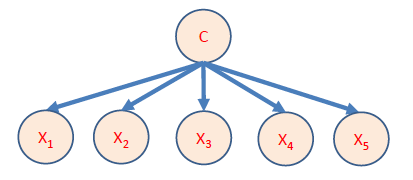
\includegraphics[scale=0.5]{bernoulliNBexample1}
  \caption{C is the class which has $x_1$ to $x_5$ features, while the lines are conditional probabilites. Notice $x_1$ to $x_5$ are assumed to be independent(Source:precept slides)}   
  \label{fig:picture}
\end{figure}


The basis of a naive bayes classifier is the conditional probability, which asks a very simple question: what is the probability that a certain random variable in our case a document, is either a positive or a negative review, given that it contains a certain sequence of words. Given a feature set of $F$ = $\mathcal \{\bm{x_1},\bm{x_2}...\bm{x_N}\}$, and a class set of $C$ = $\mathcal \{\bm{c_1},\bm{c_2}...\bm{c_N}\}$, we want to find 
\begin{equation*}
\arg\max_{c} P(C=c|F)
\end{equation*}

Using Bayes theorem, we know that, 
\begin{equation*}
P(C|x) = \frac {P(C)P(x|C)}{P(x)}
\end{equation*}

In our case the feature set contains more than one element. Hence we need to extend Bayes theorem so that C is conditioned on  all the elements of the feature set and their values. Using the chain rule of conditional probability we then can further expand the equation. However, that expanded equation can become very tractable by naively assuming that all the elements in the feature set are independent of each other. Hence the previous equation can be approximated to, 

\begin{equation*}
\alpha  \     P(C|x) = \frac {{P(C)}\prod_{i=a}^{b}P(x_i|C)}{P(x)}
\end{equation*}

However, that expanded equation can become very tractable by naively assuming that all the elements in the feature set are independent of each other. Hence the previous equation can be approximated to, Using the chain rule of conditional probability we then can further expand the equation. 

\begin{figure}[H]
  \centering
  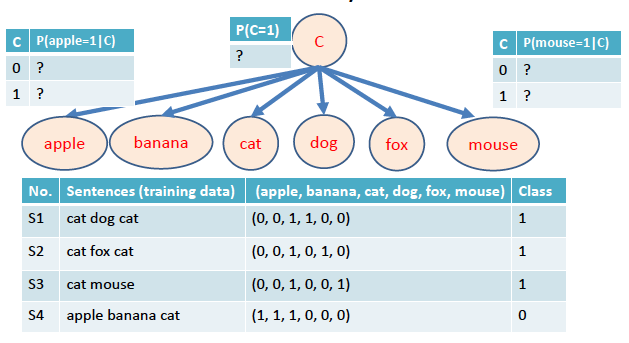
\includegraphics[scale=0.4]{bernoulliNBexample3}
  \caption{By using Naive Bayes equation as approximated above we can come up with a model that gives us the highest probabilty of a certain feature set belonging either to Class 1 or 0 (Source: precept slides)}   
  \label{}
\end{figure}



\section{Results}
\subsection{Evaluation results}
From Table~\ref{tab:classifiers} we can see that after performing a 10-fold cross validation training/testing on the whole dataset, the least sophisticated and fastest classifers namely multinomial naive bayes and bernoulli naive bayes classifiers perform better in accuracy, precision and computing time. This is to be somewhat expected as the problem that was at hand especially with the feature extraction and selection techniques I used, did not require a highly complex classifier. Even though it was not tested for this task, if feature selection was performed using support vector machine with linear kernel and $l_1$ penalty, the more complicated classifiers would begin to outperform the naive bayes classifiers. 


\begin{table}[H]
\centering
   \begin{tabular}{@{}|c|c|c|c|c|c|@{}} % Column formatting, @{} suppresses leading/trailing space 
	
   \hline

   Classifier & Accu & Prec & Recall & $F_1$ & Time (s) \\ \hline 
      MNB & 0.693 & 0.690 & 0.699 & 0.694 & 0.431 \\
       BNB & 0.694&  0.696 & 0.689 & 0.693 & 0.557\\
      SVM    &  0.686 & 0.676 & 0.713 & 0.694 & 14.431\\
        DT  &  0.677 & 0.671 & 0.696 & 0.6832 & 14.409 \\
      RT &  0.679 & 0.667 & 0.713 & 0.689 & 14.425  \\
      KNN &  0.650 & 0.699 & 0.526 & 0.600 & 21.320 \\
     \hline
   \end{tabular}
\caption{{\bf Results from six classifiers on 3000 reviews dataset.} For each classifier, we report precision, recall,  $F_1$-scores, and wall clock time in seconds for the one-versus-rest classification task with 10-fold cross validation.}
   \label{tab:classifiers}
\end{table}

I used 10-fold cross validation to tune hyperparameters for the k-nearest neighbours classifier. It is clear from the  Figure~\ref{fig:sub1} and Figure~\ref{fig:sub2} that as the hyperparameter value increased, the accuracy of the classifier generally decreases. From the figures, I was able to determine tht 5 is the optimal hyperparamater for the classifier together with the given data set.  It should be noted that I tuned the hyperparameter without including the test data set. I included the test data set only after the hyperparameter had been tuned. 

Moreover, as can be seen from Figure~\ref{fig:sub3} and Figure~\ref{fig:sub4}, there is a general but very slight decrease of accuracy as you increase the hyperparameter for a random forest classifier. Moreover, with an increase of the hyperparameter there was an increase of computational time taken.As can be seen from the figures, it seems like 14 is the optimal hyperparameter value for the problem we are facing. I used 14 to evalute the performance of the random forest classifier. 

\begin{figure}[H]
\centering
\begin{subfigure}{.4\textwidth}
  \centering
  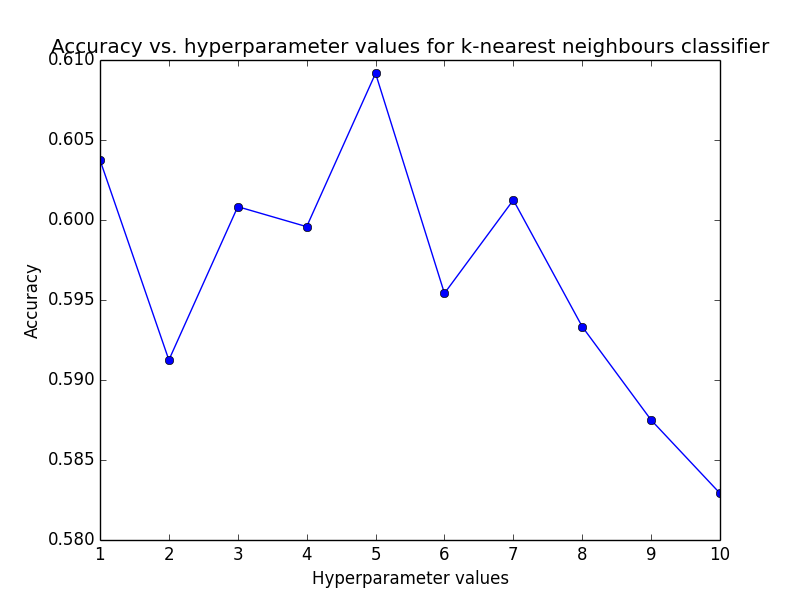
\includegraphics[width=.9\linewidth]{hyperparameter_knn_1_10.png}
  \caption{hyperparamter values between 1-10}
  \label{fig:sub1}
\end{subfigure}%
\begin{subfigure}{.4\textwidth}
  \centering
  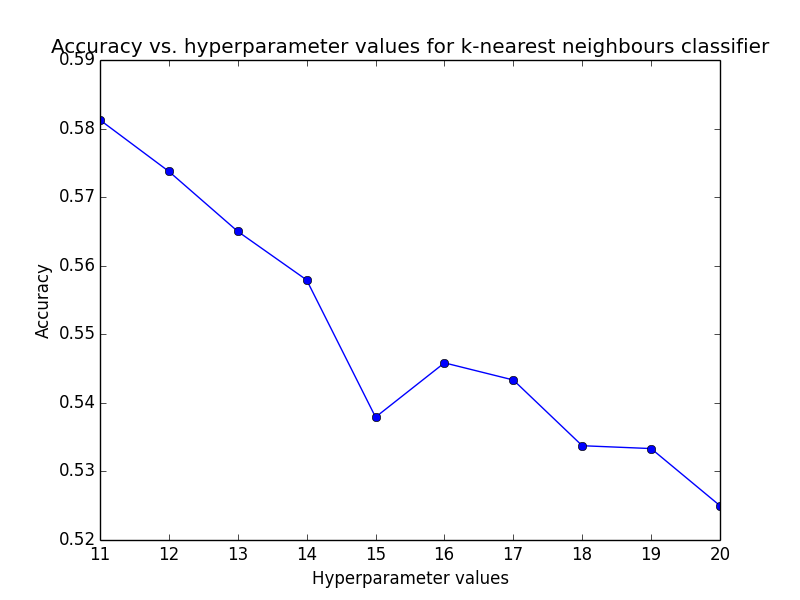
\includegraphics[width=.9\linewidth]{hyperparameter_knn_11_20.png}
  \caption{hyperparamter values between 11-20}
  \label{fig:sub2}
\end{subfigure}
\caption{Accuracy vs. hyperparameter values for k-nearest neighbours classifier}
\label{fig:test1}
\end{figure}

\begin{figure}[H]
\centering
\begin{subfigure}{.4\textwidth}
  \centering
  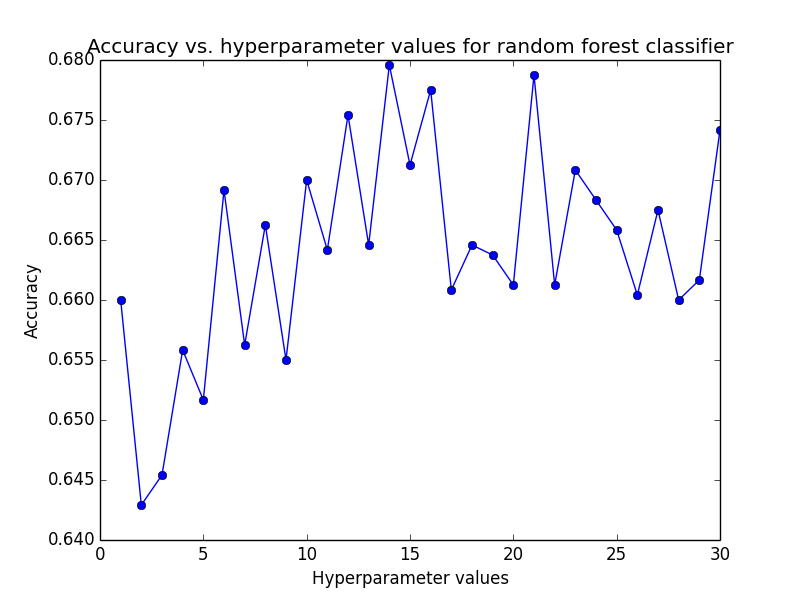
\includegraphics[width=.9\linewidth]{hyperparameter_forest_1_30.png}
  \caption{hyperparamter values between 0-30}
  \label{fig:sub3}
\end{subfigure}%
\begin{subfigure}{.4\textwidth}
  \centering
  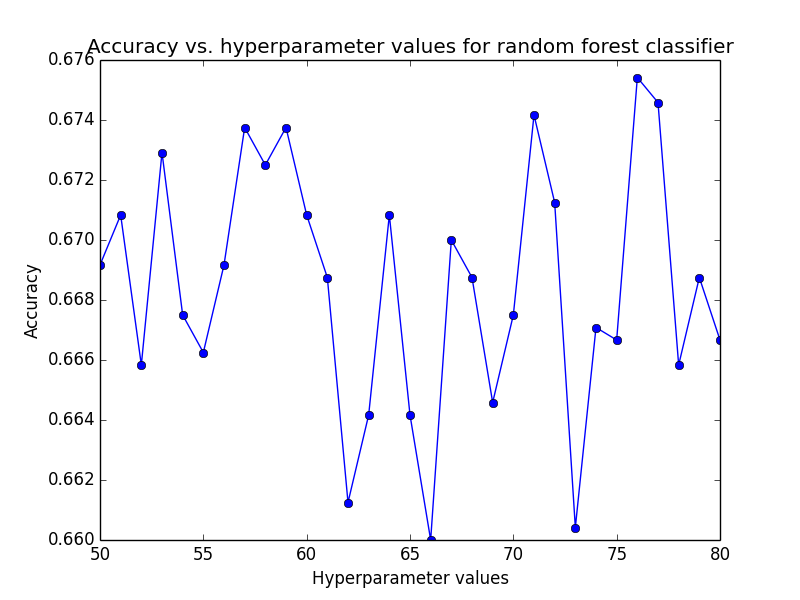
\includegraphics[width=.9\linewidth]{hyperparameter_forest_50_81.png}
  \caption{hyperparamter values between 50-80}
  \label{fig:sub4}
\end{subfigure}
\caption{Accuracy vs. hyperparameter values for random forest classifier}
\label{fig:test2}
\end{figure}



\subsection{Computational speed}

As can be seen from  except for multinomial naive bayes and bernoulli naive bayes, all the rest of the classifiers  take a significant amount of time to train. The time given is the amount of time taken to train a 3000 document data set using 10-fold cross validation technique. The fastest classifiers are as expected Multinomial Naive Bayes and Bernoulli Naive Bayes. They are the fastest amongst the classifiers because the number of parameters required is linear to the number of features in a learning problem. "Moreover,  Maximum-likelihood training can be done by evaluating a closed-form expression,[1]which takes linear time."(Wikipedia)\cite{Russell2003}







\section{Discussion and Conclusion}
In this work, I compared 6 classifiers to predict if a certain review had a positive or a negative sentiment. I found that all six classifiers performed relatively closely in terms of precision and recall values but the time taken to train and test data was significantly lower for the naive bayes classifiers. 

If we were to perform more rigorous feature selection, the more complicated classifiers would perform better in precision and recall but also on time of computation. Moreover, future work can be done by focusing on the feature extraction and feature selection process, further tuning the response of each classifier so as to get the best result.  
%\subsubsection*{Acknowledgments}


\bibliography{ref}
\bibliographystyle{plos2015}

\end{document}
